\chapter{Evaluation}
\label{ch:evaluation}

After we finished implementing our system, we began to evaluate our system
in terms of performances of response speed and memory usage. To evaluate
the system, we need some decent amount of sample data, so here we
introduce the standard name list.

\section{Introducing standard name list}
\label{sec:stdname}

In subsection \ref{sub:lookuptable}, we mentioned Robert Edwin Matheson,
who developed a classification of Irish names. He classified
the surnames in Ireland into 2091 groups. Adam Winstanley's work
on this classification \cite[]{adamw} looked through these groups
and came up with a total 12,944 names in this classification.
We use all these names to build up our lookup table (section \ref{sec:lookuptable}).

We also decide to use all these records as a standard name list,
for example, a client may want to match the \emph{base name} `MONAHAN'
for all any possible matching \emph{to-match names}. A client has
an option to choose to match `MONAHAN' with all 12,944 names in
our standard list.

For web service clients, specify \texttt{standard\_list} as
\texttt{true}, \texttt{t}, or \texttt{1} to use the standard list.
For example in listing \ref{lst:json_std}, note that
\texttt{to\_match\_names} is left blank and \texttt{standard\_list} value is 1.

\begin{minipage}{\linewidth}
  \begin{lstlisting}[language={json}, label={lst:json_std}, caption={Sample \texttt{JSON} with a standard name list option.}]
{
  "base_names":"Monahan",
  "to_match_names":"",
  "matching_algorithms":{
    "1":{"name":"LookupTable", "weight":"10"},
    "2":{"name":"LevenshteinDistance", "weight":"1"},
    "3":{"name":"Soundex", "weight":"3"},
    "4":{"name":"IrishSoundex", "weight":"6"}
  },
  "threshold":"0",
  "standard_list":"1"
}
\end{lstlisting}
\end{minipage}

For web interface clients, check the ``Use standard list'' checkbox
to use the standard list, as shown in figure \ref{fig:wi_std}.

\begin{figure}[H]
\centering
\captionsetup{justification=centering}
\makebox[\textwidth][c]{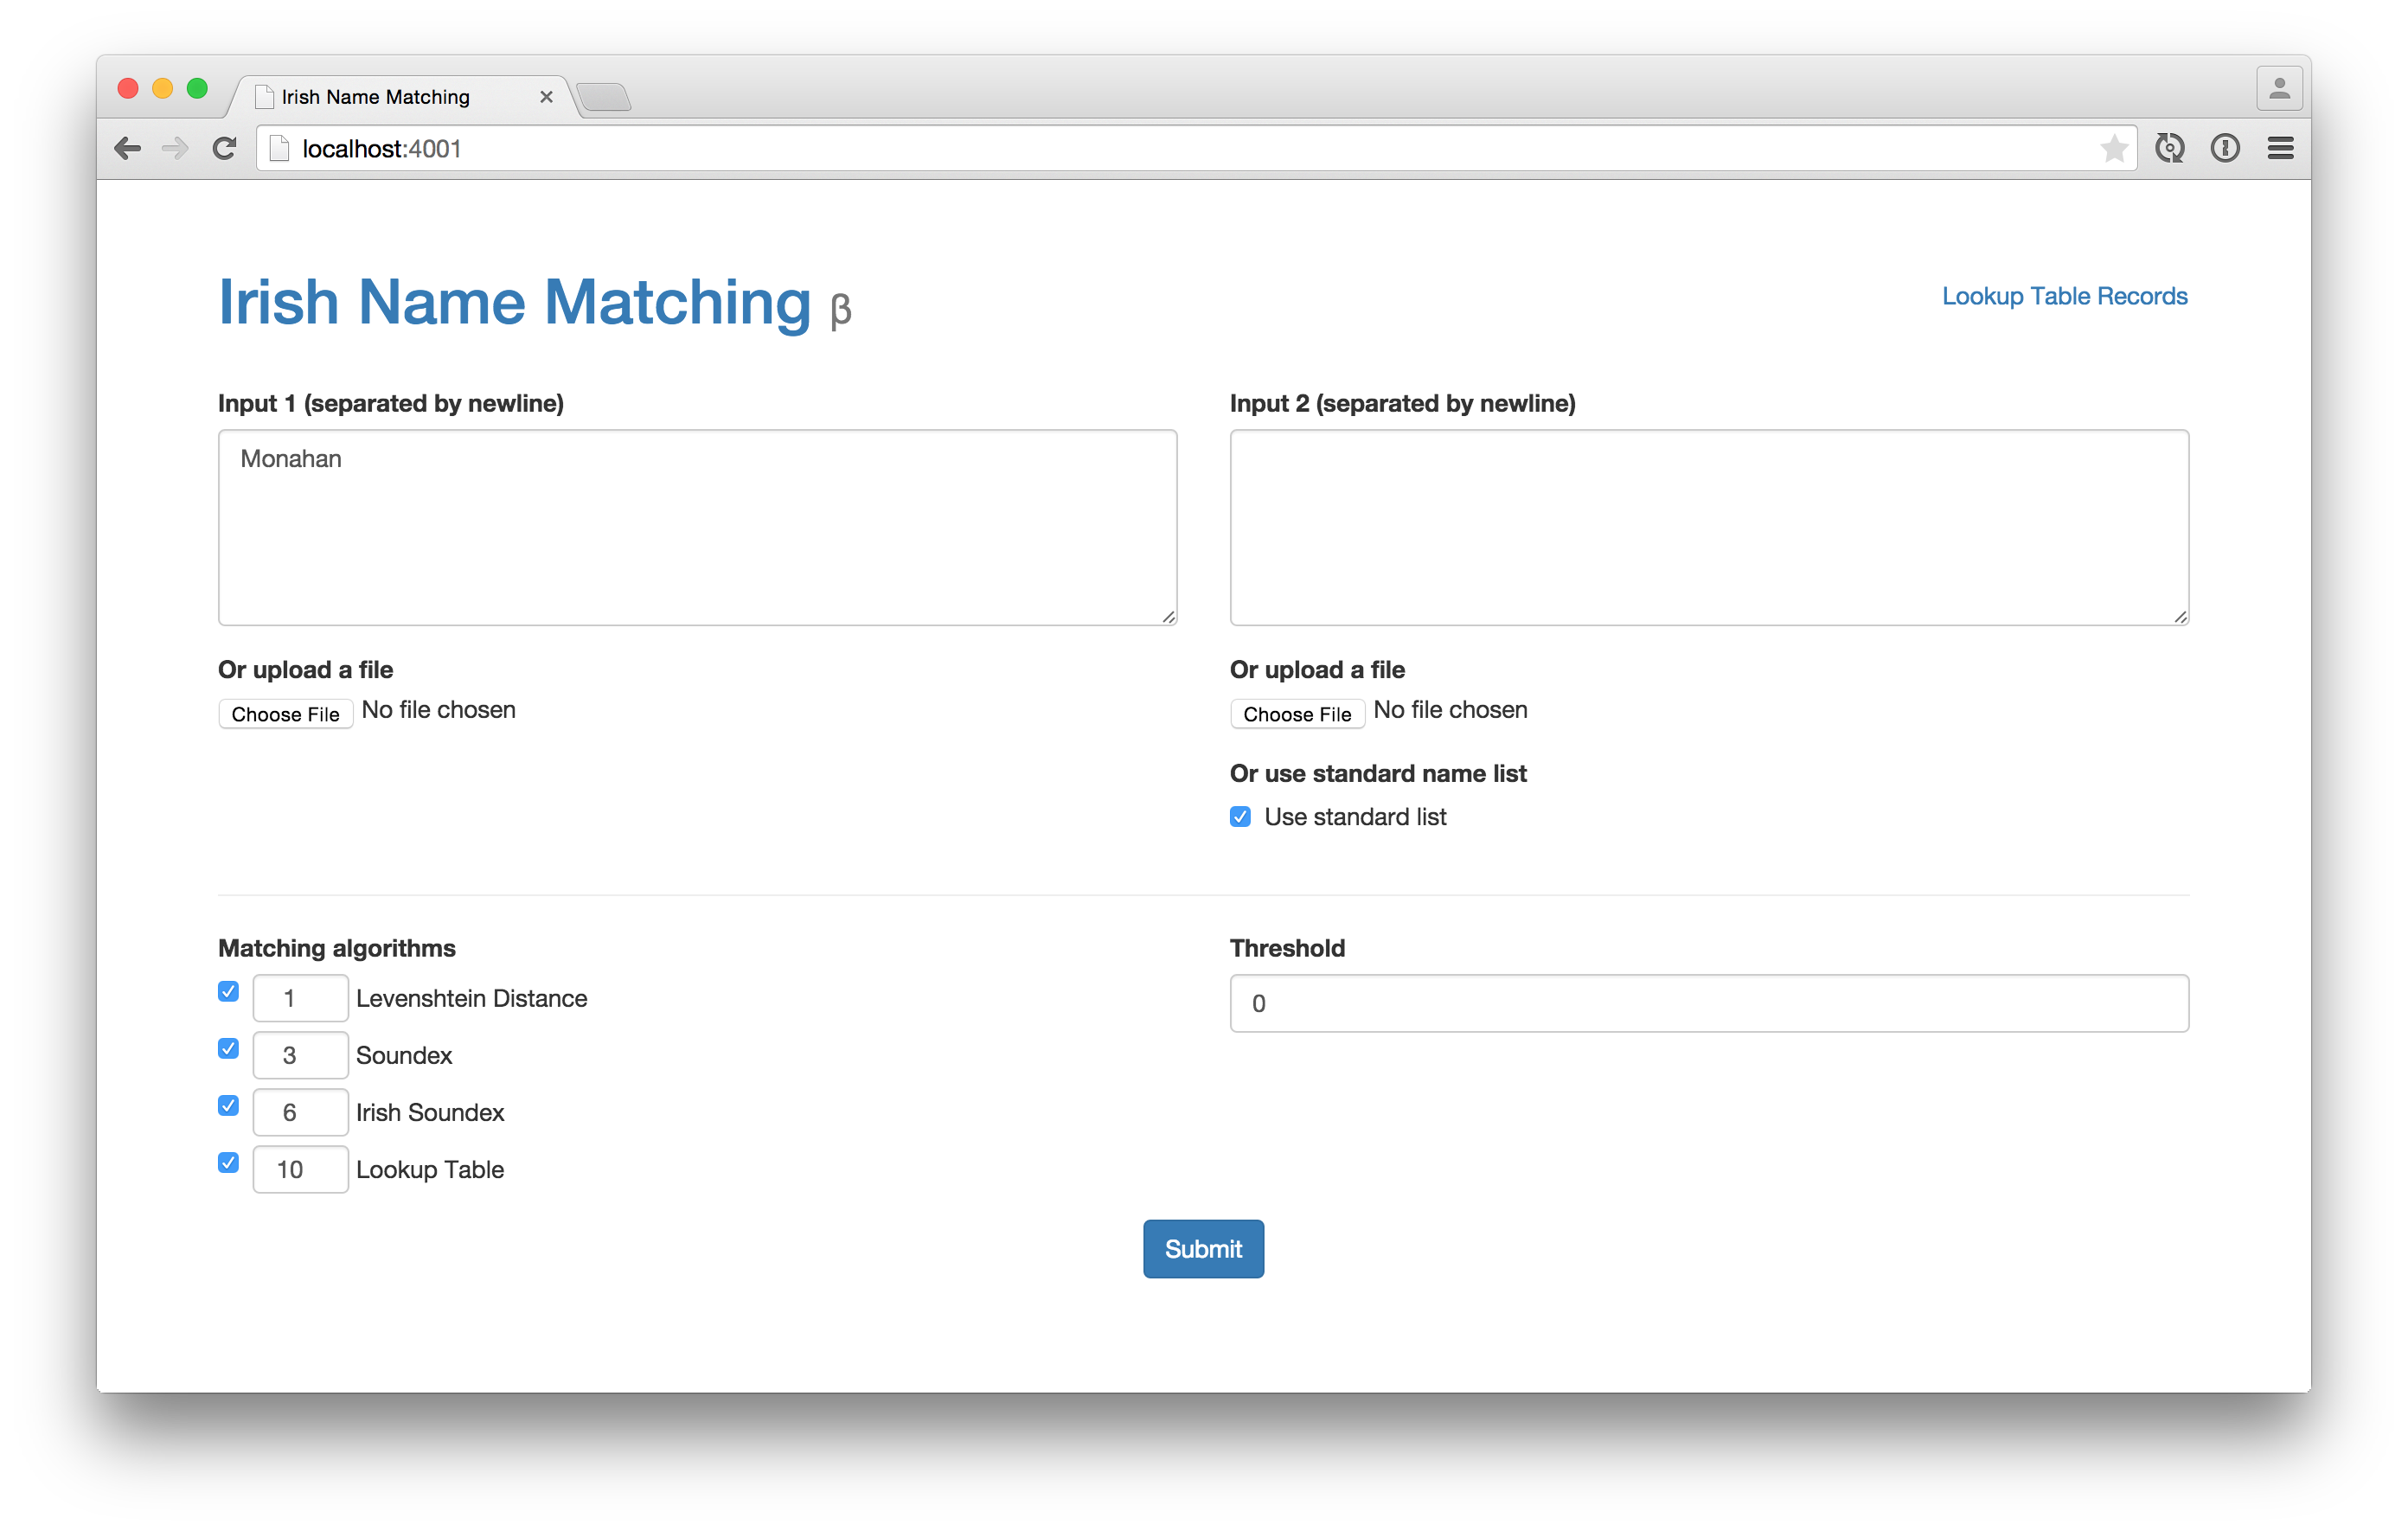
\includegraphics[width=16cm]{gfx/wi_std}}
\caption{Web interface with a standard name list option.}
\label{fig:wi_std}
\end{figure}

Using a standard name list option generates many results.
Client is suggested also specify a proper threshold (section \ref{sec:threshold})
to discard irreverent results.

In listing \ref{lst:json_std_out} is a result of matching between
\emph{base name} `MONAHAN' and the standard name list, using threshold as 0.9.
Results' detailed scores are truncated for readability.

\begin{minipage}{\linewidth}
  \begin{lstlisting}[language={json}, label={lst:json_std_out}, caption={Results of matching \emph{base name} `MONAHAN' with a standard name list.}]
[
  {
    "base_name": "MONAHAN",
    "to_match_names": [
      {
        "to_match_name": "MONAHAN",
        "overall_weighted_score": 1,
        ..
      },
      {
        "to_match_name": "MOYNAHAN",
        "overall_weighted_score": 0.994,
        ..
      },
      {
        "to_match_name": "MONOHAN",
        "overall_weighted_score": 0.993,
        ..
      },
      {
        "to_match_name": "MONEHAN",
        "overall_weighted_score": 0.993,
        ..
      },
      {
        "to_match_name": "MOYNIHAN",
        "overall_weighted_score": 0.988,
        ..
      },
      {
        "to_match_name": "MOYNAN",
        "overall_weighted_score": 0.979,
        ..
      }
    ]
  }
]
\end{lstlisting}
\end{minipage}

\section{Test environment setup}
\label{sec:testenv}

We run, test, and profile our system locally, using these following
environmental setup.

\begin{description}
  \item[Test machine:] MacBook Pro (Retina, 13-inch, Mid 2014).
    \begin{itemize}
      \item Processor -- 2.6 GHz Intel Core i5
      \item Memory -- 8 GB 1600 MHz DDR3
      \item Hard disk -- APPLE SSD SM0256F
    \end{itemize}
  \item[Ruby:] 1.9.3p125 (2012-02-16 revision 34643) with
    GC-Patched MRI\footnote{Installing GC-Patched MRI \cite[]{perftest}.}.
  \item[Ruby on Rails:] version 4.2.0.
  \item[Database:] PostgreSQL version 9.3.5.
  \item[Profiling tools:] rails-perftest \cite[]{perftest} 0.0.6.
\end{description}

\section{Response speed}

We test response speed of our system by matching \emph{base name} `SMITH'
with the standard name list of total 12,944 names. Each matching algorithm
is tested separately first and then altogether at last.

Listing \ref{lst:resp_json} is our \texttt{JSON} setup for response speed
testing. Matching algorithms are varies between each scenario
and all use default weights.

\begin{minipage}{\linewidth}
  \begin{lstlisting}[label={lst:resp_json}, caption={\texttt{JSON} setup for performance testing.}]
{
  "base_names":"Smith",
  "to_match_names":"",
  "matching_algorithms":{
    ..
  },
  "threshold":"0",
  "standard_list":"1"
}
\end{lstlisting}
\end{minipage}

To conduct testing, we use \emph{rails-perftest} \cite[]{perftest} to
run our test cases. Table \ref{table:speed_res} shows the test result in response speed aspect.

\begin{table}[H]
  \myfloatalign
  \setlength{\tabcolsep}{0.3cm}
  \begin{tabular}{r c}
    \toprule
    \tableheadline{Matching algorithms} & \tableheadline{Response speed (ms)} \\
    \midrule
    Levenshtein distance & 1,337 \\
    Soundex & 2,024 \\
    Irish soundex & 2,456 \\
    Lookup table & 24,293 \\
    \midrule
    All 4 algorithms & 28,786 \\
    \bottomrule
  \end{tabular}
  \caption{Response speed for each matching algorithms.}
  \label{table:speed_res}
\end{table}

From the results, Levenshtein distance is the fastest matching algorithm
because it has the simplest logic among the four. Soundex and Irish soundex
are second and third because they involve more string converting logic,
and Irish soundex has more steps. Lastly, lookup table involves many
database queries so that makes it much more slower than the rest.

\section{Memory usage}

We also test memory usage of our system by matching \emph{base name} `SMITH'
with the standard name list of total 12,944 names. Each matching algorithm
is tested separately first and then altogether at last.

Listing \ref{lst:resp_json} is still our \texttt{JSON} setup for response speed
testing. Matching algorithms are varies between each scenario
and all are using default weights. Table \ref{table:mem_res} shows
the test result in memory usage aspect.

\begin{table}[H]
  \myfloatalign
  \setlength{\tabcolsep}{0.3cm}
  \begin{tabular}{r c}
    \toprule
    \tableheadline{Matching algorithms} & \tableheadline{Memory usage (bytes)} \\
    \midrule
    Levenshtein distance & 48,518,621 \\
    Soundex & 53,066,150 \\
    Irish soundex & 69,534,598 \\
    Lookup table & 244,302,744 \\
    \midrule
    All 4 algorithms & 373,544,727 \\
    \bottomrule
  \end{tabular}
  \caption{Memory usage for each matching algorithms.}
  \label{table:mem_res}
\end{table}

From the results, memory usage for each algorithm follows response speed fashion.
Levenshtein distance and two soundexes use much less memory
compared to lookup table.
